\documentclass[journal,onecolumn]{IEEEtran}
%\usepackage[left=2.2cm,right=2.2cm,top=2.5cm,bottom=2.5cm]{geometry}
\usepackage[utf8]{inputenc}
\usepackage{minted}
\usepackage{booktabs}
\usepackage{commath}
\usepackage{float}
\usepackage{mathtools}
\usepackage{color}
\usepackage{amsthm}
\usepackage{parskip}


\usepackage[binary-units=true]{siunitx}

\newcommand{\py}[1]{\mintinline{python}{#1}}

\title{Artificial Intelligence (\texttt{LINGI2261}) \\ Assignment 3 --- Group 13}
\author{Martin Braquet, Gilles Peiffer}
\date{November 27, 2019}

\begin{document}

\maketitle

\section{Alpha-Beta Search}
Figure~\ref{fig:minimax} can be obtained by applying the minimax algorithm to the tree given in the statement.
\subsection{MiniMax Algorithm}
\begin{figure}[H]
 \centering
 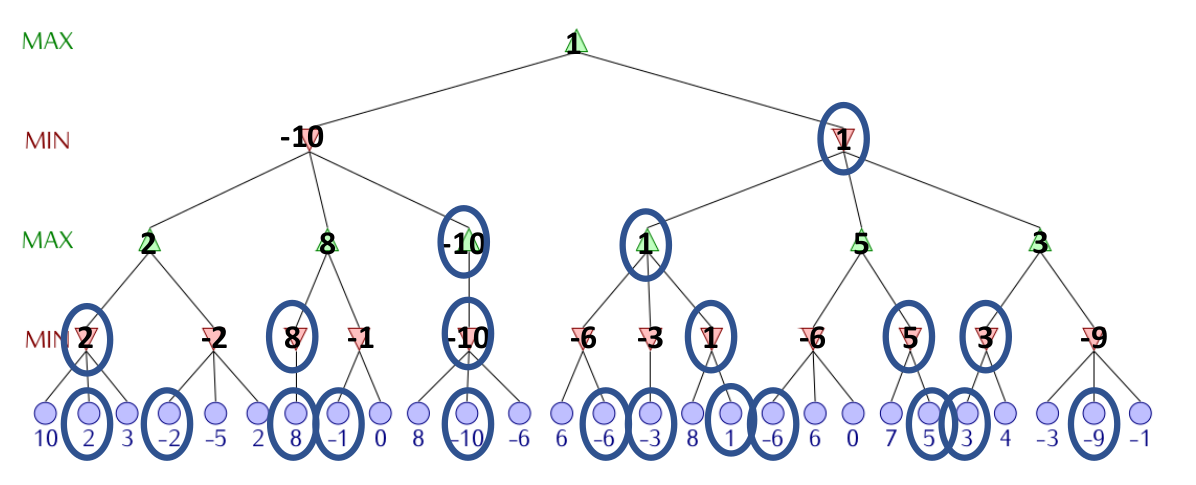
\includegraphics[width=\textwidth]{img/MiniMax.png}
 \caption{Minimax algorithm}
 \label{fig:minimax}
\end{figure}
One notices that nodes in the ``MAX'' nodes simply take on the highest value among their child nodes, whereas ``MIN'' nodes take on the lowest value among their child nodes.

\subsection{Alpha-Beta Algorithm (Left To Right)}
Using a technique called ``Alpha-Beta pruning'', the number of nodes which have to be explored can be reduced (though it stays exponential in the worst case).
This is shown in Figures~\ref{fig:alphabeta} and \ref{fig:alphabeta_reverse}.
\begin{figure}[H]
 \centering
 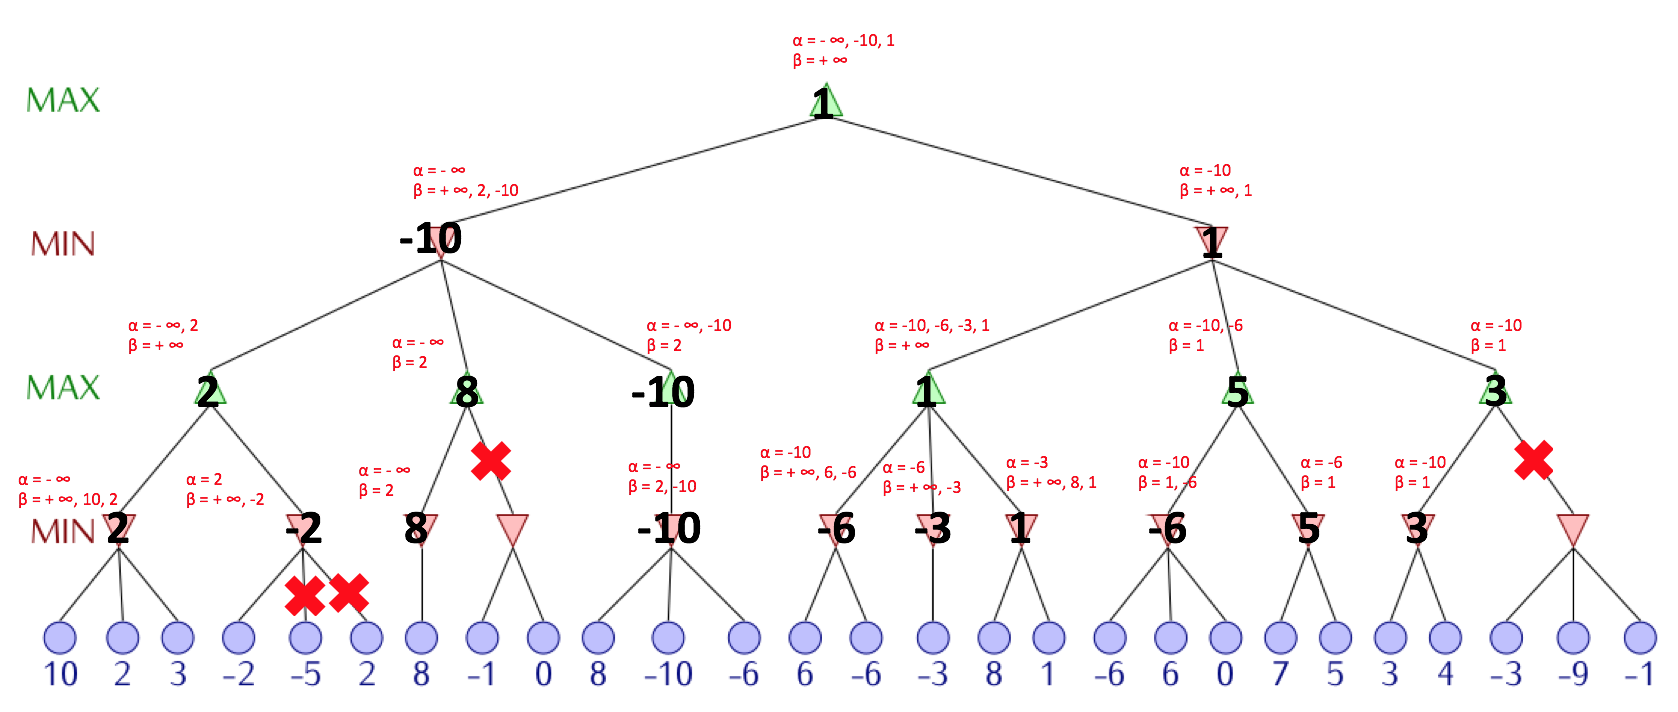
\includegraphics[width=\textwidth]{img/Alphabeta.png}
 \caption{Alpha-Beta algorithm (left to right)}
 \label{fig:alphabeta}
\end{figure}
Every red cross denotes a pruning operation.
For example, the two leftmost prunings are possible because no matter what values \(x\) and \(y\), they give, their parent node is going to take on value \(\min\{-2, x, y\} \le -2 < 2\), which is the value which is going to be conserved when moving up to the ``MAX'' node on the row above.
The values of \(\alpha\) and \(\beta\) are used to keep track of when a subtree can be pruned.

\subsection{Alpha-Beta Algorithm (Right To Left)}
\begin{figure}[H]
 \centering
 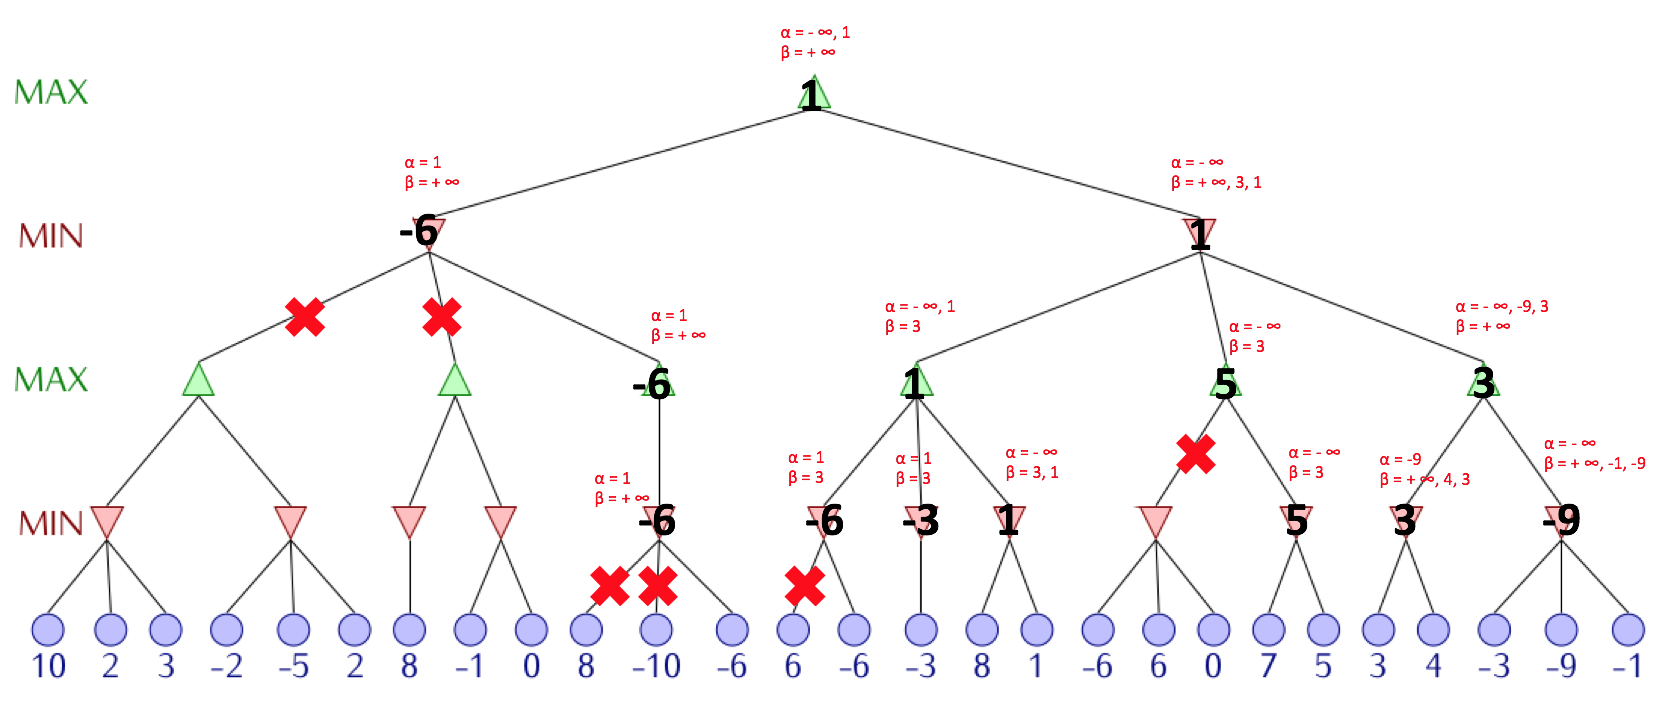
\includegraphics[width=\textwidth]{img/Alphabeta_reverse.png}
 \caption{Alpha-Beta algorithm (right to left)}
 \label{fig:alphabeta_reverse}
\end{figure}


\subsection{Alpha-Beta Algorithm (Ordered)}
Using this pruning algorithm, it is possible to find an ordering of the nodes which, when used to determine which nodes are explored first, minimizes the amount of nodes that need to be explored.
This optimal tree is shown in Figure~\ref{fig:alphabeta_ordered}, assuming a left-to-right exploration.
To obtain this tree, one needs to order nodes in ascending order on MAX levels and in descending order on MIN levels.
\begin{figure}[H]
 \centering
 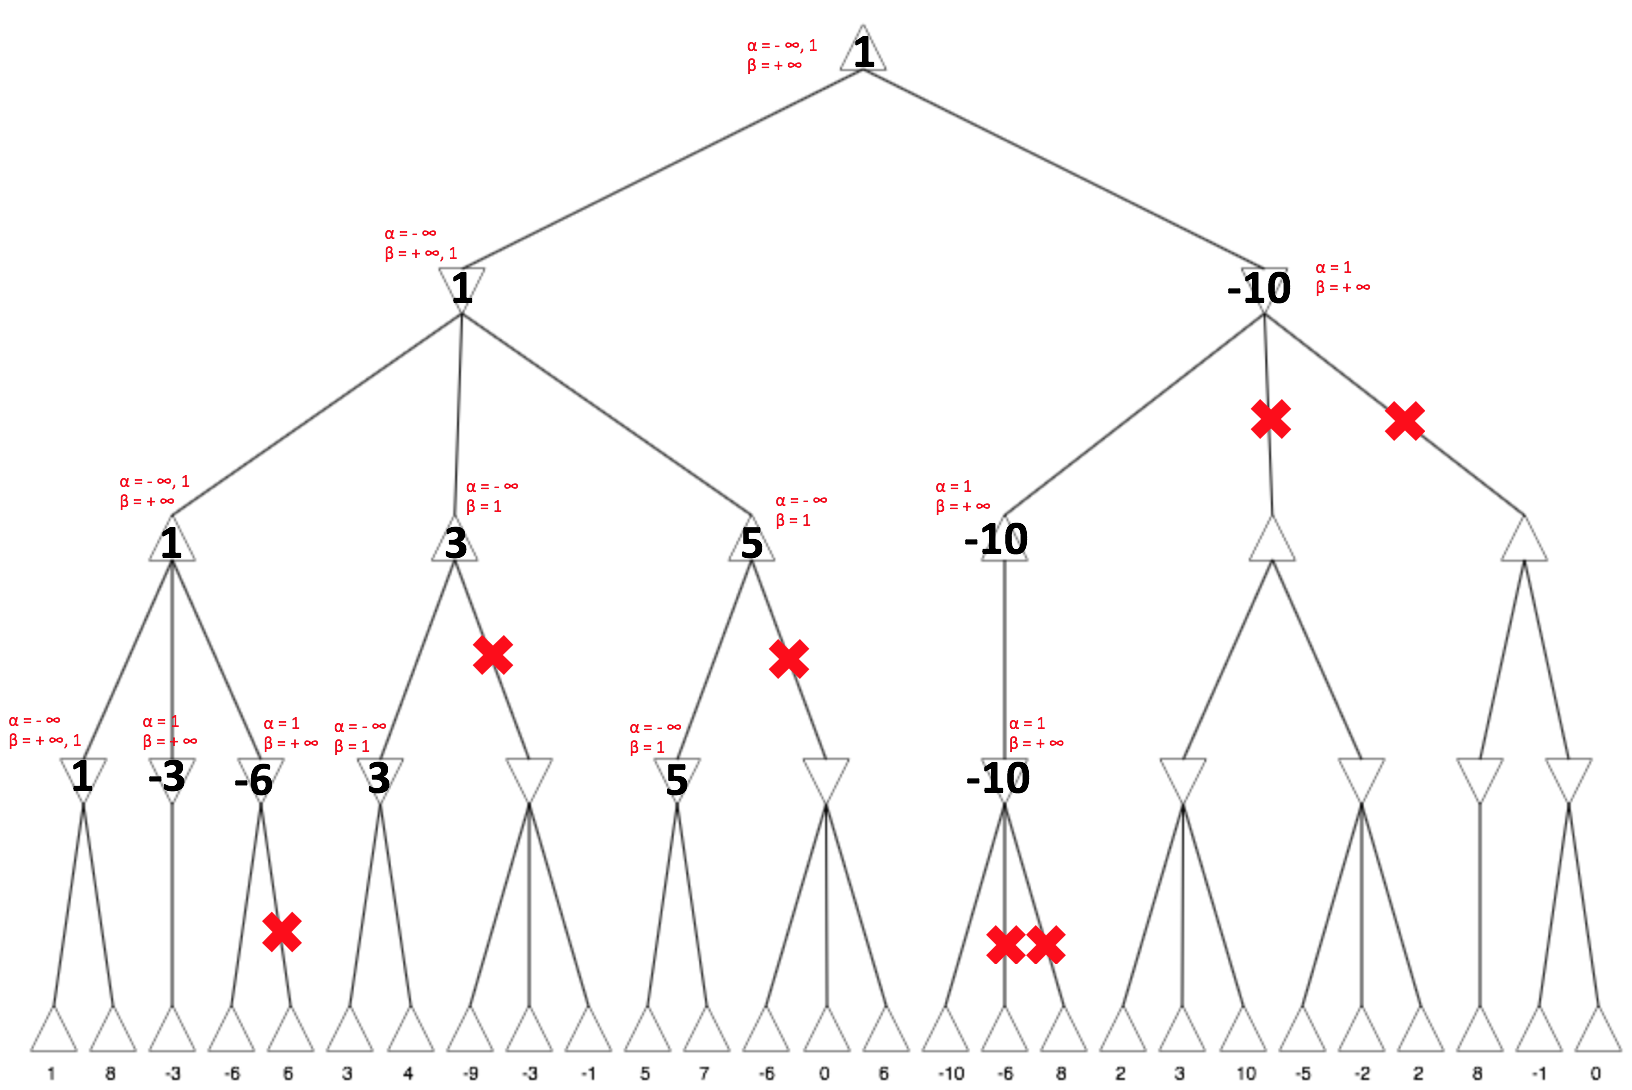
\includegraphics[width=\textwidth]{img/Alphabeta_ordered.png}
 \caption{Alpha-Beta algorithm}
 \label{fig:alphabeta_ordered}
\end{figure}

\subsection{Alpha-Beta For More Than Two Players}
For games with more than two players, each node is associated with a tuple giving the value of each player for that state.

Tree pruning is possible if there is an upper bound on the sum of all components of this tuple, and if there is a lower bound on the values of each component.
We define the sum $S$ as the global upper bound on the sum of all components of the \(N\)-tuple, and all components are assumed to be nonnegative. 

The conditions \py{v <= alpha} and \py{v >= beta} are now given by \py{Best[Player] >= Bound} where the bound equals the sum $S$ minus the last best node of the upper layer.
Indeed, let us take a player 1 from the upper layer which is ensured to get a value of at least $x$ for his layer: $(\ge x, \dots, \dots)$. Then, if player 2 from the lower layer unveils a child with more than $S - x$ for its own value, it will result in a score of $(\le x, \ge S - x, \dots)$. Thus, all the remaining children can be dropped since player 1 knows that these children will be chosen by player 2 only if the value of player 1 is less than $x$. \cite{multiplayer}

\begin{figure}[H]
 \centering
 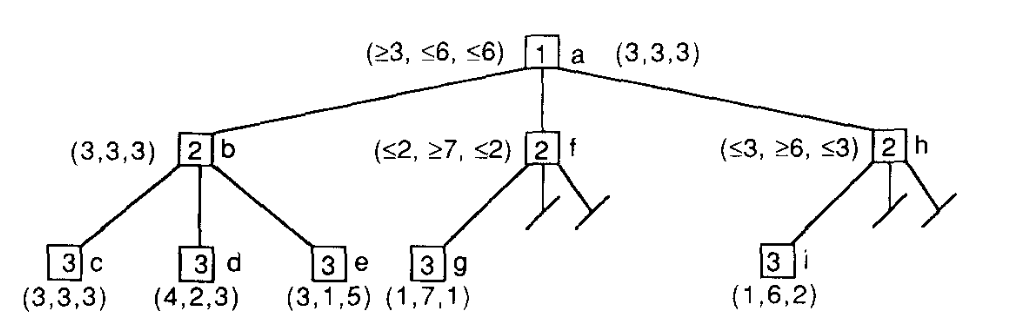
\includegraphics[width=0.7\textwidth]{img/multiplayer.png}
 \caption{Shallow pruning in three-player game tree \cite{multiplayer}}
 \label{fig:multiplayer}
\end{figure}


\section{Squadro}

\subsection{Comparison Of Two Evaluation Functions}
One would expect that the new evaluation will work better since it takes into account the opponent, and will thus try to prevent them from winning, for example, by killing their pawns.
The old agent is not able to deliberately kill the opponent, consequently decreasing its chances of winning.

However, the yellow player still always wins in the four possible starting configurations because it begins with the best pawns at the center, progressing by steps of three.
The yellow player rapidly puts these pawns on the other side, which then form a barrier for the opponent's progress.
Thus, when the depth of the minimax algorithm is not sufficient, the new basic agent is not good enough to overcome the yellow player's innate advantage.

\subsection{Cut-Off Function}
The \emph{depth} in the \py{minimax.py} implementation is the number of steps along the path from the root node to a node in the layer where we stop the tree search and evaluate the node.

When the depth increases, the new basic agent is able to win even when playing as the red player because it can now predict and find a counter-attack against the yellow barrier.
The new basic agent wins for all starting configurations when the depth is higher than six.

Since the Squadro contest has a time limit, one needs to select the time allowed for each move.
There exist different methods to choose the maximum time allowed for each search, but an interesting option is to decrease the allotted time throughout the game in order to prevent exceeding the limit.
Indeed, one can split the time for each move $t_\textnormal{move}$ according to the next formula:
\[
    t_\textnormal{move} = 
    \left\{
    \begin{array}{ll}
      0.2 \: t_\textnormal{left}^2, & \mathrm{if}\quad t_\textnormal{left}\leq \min\{\SI{100}{s}, t_\textnormal{total}/3\}, \\
      20, & \mathrm{otherwise.} \\
    \end{array} 
    \right.
\]
where $t_\textnormal{left}$ is the remaining amount of time for the considered player and \(t_\textnormal{total}\) is the initial time limit.
One can notice that the allowed time goes to zero as the remaining time drops, as expected.

Using iterative deepening is a good choice to stop the algorithm during its search.
Iterative deepening depth-first search is a search method which iteratively performs a depth-limited depth-first search using the minimax algorithm, starting from a limit depth of one, up to some predefined value.
By recording the optimal path at each depth, the moves can be ordered in such a way as to minimize the total search time, coompensating for the (asymptotically negligible) cost of searching with lower depth limits.

The depth is chosen so that the algorithm gives good results, for instance eight.
However, when time runs out, the program returns the move selected by the deepest completed search.

The cut-off function, which reflects the moment when we need to stop the search, is activated when one of the following three conditions is true:
\begin{enumerate}
 \item \py{depth > self.current_depth}: the depth of the analyzed node is higher than the maximum depth,
 \item \py{state.game_over_check()}: the game is over,
 \item \py{time() - self.start_time > self.max_time}: the time elapsed during this search has exceeded the maximum allowed period for this search.
\end{enumerate}

\subsection{Evaluation Function}
In the figure presented in the instructions, the yellow basic agent will move its pawn number 3 since it will lead to the highest value of its evaluation function: the sum over all pawns of each's advancement.
However, it is clear that this is not the best possible move, since moving pawn number 4 would make it win the game.
A stronger heuristic thus has to take into account that a player wins if only four of their pawns return to their initial position.
In practice, we reduce this progress evaluation to only the four most advanced pawns, bringing a more cogent representation of the state.

Other weak points of the evaluation function of the basic agents are
\begin{itemize}
	\item \textcolor{red}{To complete}
	\item 
	\item 
\end{itemize}
In addition to the sum of each pawn’s advancements, the following features are detailed below.

\begin{itemize}
 \item \textcolor{red}{To complete}
 \item 
 \item 
\end{itemize}

The improved evaluation function

\subsection{Contest}
For the contest agent, we have opted for 

\bibliographystyle{unsrt}
\bibliography{bib.bib}

\end{document}
